\section{Estudo com Redes Neuronais}
Sendo que o pressuposto das Redes Neuronais é que tenham um bom desempenho, em termos da qualidade da prestação de modelos treinados usando o mesmo, foi a primeira abordagem que decidimos dar ao problema.

\subsection{Estrutura usada}
Apesar do \textit{dataset} ter dimensões consideráveis para o \textit{hardware} disponível, consideramos que este problema consegue ser resolvido com uma rede neuronal "normal". O uso de uma rede convolucional neste problema acaba por ser evitado, pois na fase de pré-processamento existem métodos de selecção de \textit{features} suficientes para o modelo ter uma performance boa, não sendo necessário que o modelo tenha a responsabilidade de fazer a procura de \textit{features}.
Então após a experimentação de alguns valores relativos ao número de neurónios e número de \textit{hidden layers} consideramos uma rede neuronal com as seguintes características:

Input \textrightarrow{} 200 Neurónios \textrightarrow{} 100 Neurónios \textrightarrow{} Output

Para além disso, a inicialização dos \textit{weights} foi feita usando o  \texit{glorot uniform initializer} \cite{Glorot_Uniform}. Os valores dos hiperparâmetros usado foram:
\begin{itemize}
    \item Número de \textit{features} (termos do vocabulário): 500-600
    \item Número de \textit{epochs} = 200
    \item \textit{Batch size} = 500
    \item \textit{Activation function} 
        \begin{itemize}
            \item \textit{Hidden Layers}: \textit{Relu} \cite{relu_function}
            \item \textit{Output Layer}: \textit{Softmax} \cite{softmax_function}
        \end{itemize}
    \item \textit{Optimizer}: \textit{Adam} \cite{adam_optimizer}
    \item \textit{Loss function}: \textit{Categorical crossentropy} \cite{categorical_crossentropy_optimizer}
\end{itemize}


Desde o inicio da implementação deste modelo foi usado o processo de treino-validação utilizando o \textbf{\textit{K-Fold Cross validation}}. Este método tem um parâmetro k que define o número de divisões que o conjunto será sujeito, cada porção segmentada é intitulada de \textit{fold}. No processo de treino todos os \textit{folds} são usados para teste uma vez, sendo que os outros restantes k-1 \textit{folds} são usados para o processo de treino. Neste estudo, o valor de \textit{k} definindo foi 5 (\textbf{\textit{K\textunderscore{fold}} com 5 \textit{splits}}).
Ainda foi adicionado um \textit{callback} de \textit{Early stopping} com objectivo de suspender o treino quando o parâmetro a ser monitorizado (neste caso o \textit{validation accuracy}) para de melhorar.


\subsection{Resultados obtidos}

Após as condições definidas anteriormente decidimos então testar a performance do modelo. 
Obtivemos então os seguintes valores de \textit{accuracy}, após retreino do modelo:

\begin{itemize}
        \item \textit{Train Score}: 0.82
        \item \textit{Test Score}: 0.71
\end{itemize}


Como se pode observar pelos resultados e pelos gráficos \ref{diagram:accuracy_fold_first} e \ref{diagram:accuracy_retrain}, o modelo tem tendência a realizar o fenómeno de \textit{overfit} e portanto as próximas subsecções têm como objectivo explicar os mecanismos usados para evitar este fenómeno. Apenas de salientar que devido ao \textit{callback} de  \textit{early stopping}, o treino é parado pois a \textit{accuracy} do conjunto de validação não aumenta, o que acaba por evitar uma maximização do fenómeno de \textit{overfit}.



\begin{figure}[t]
\begin{center}
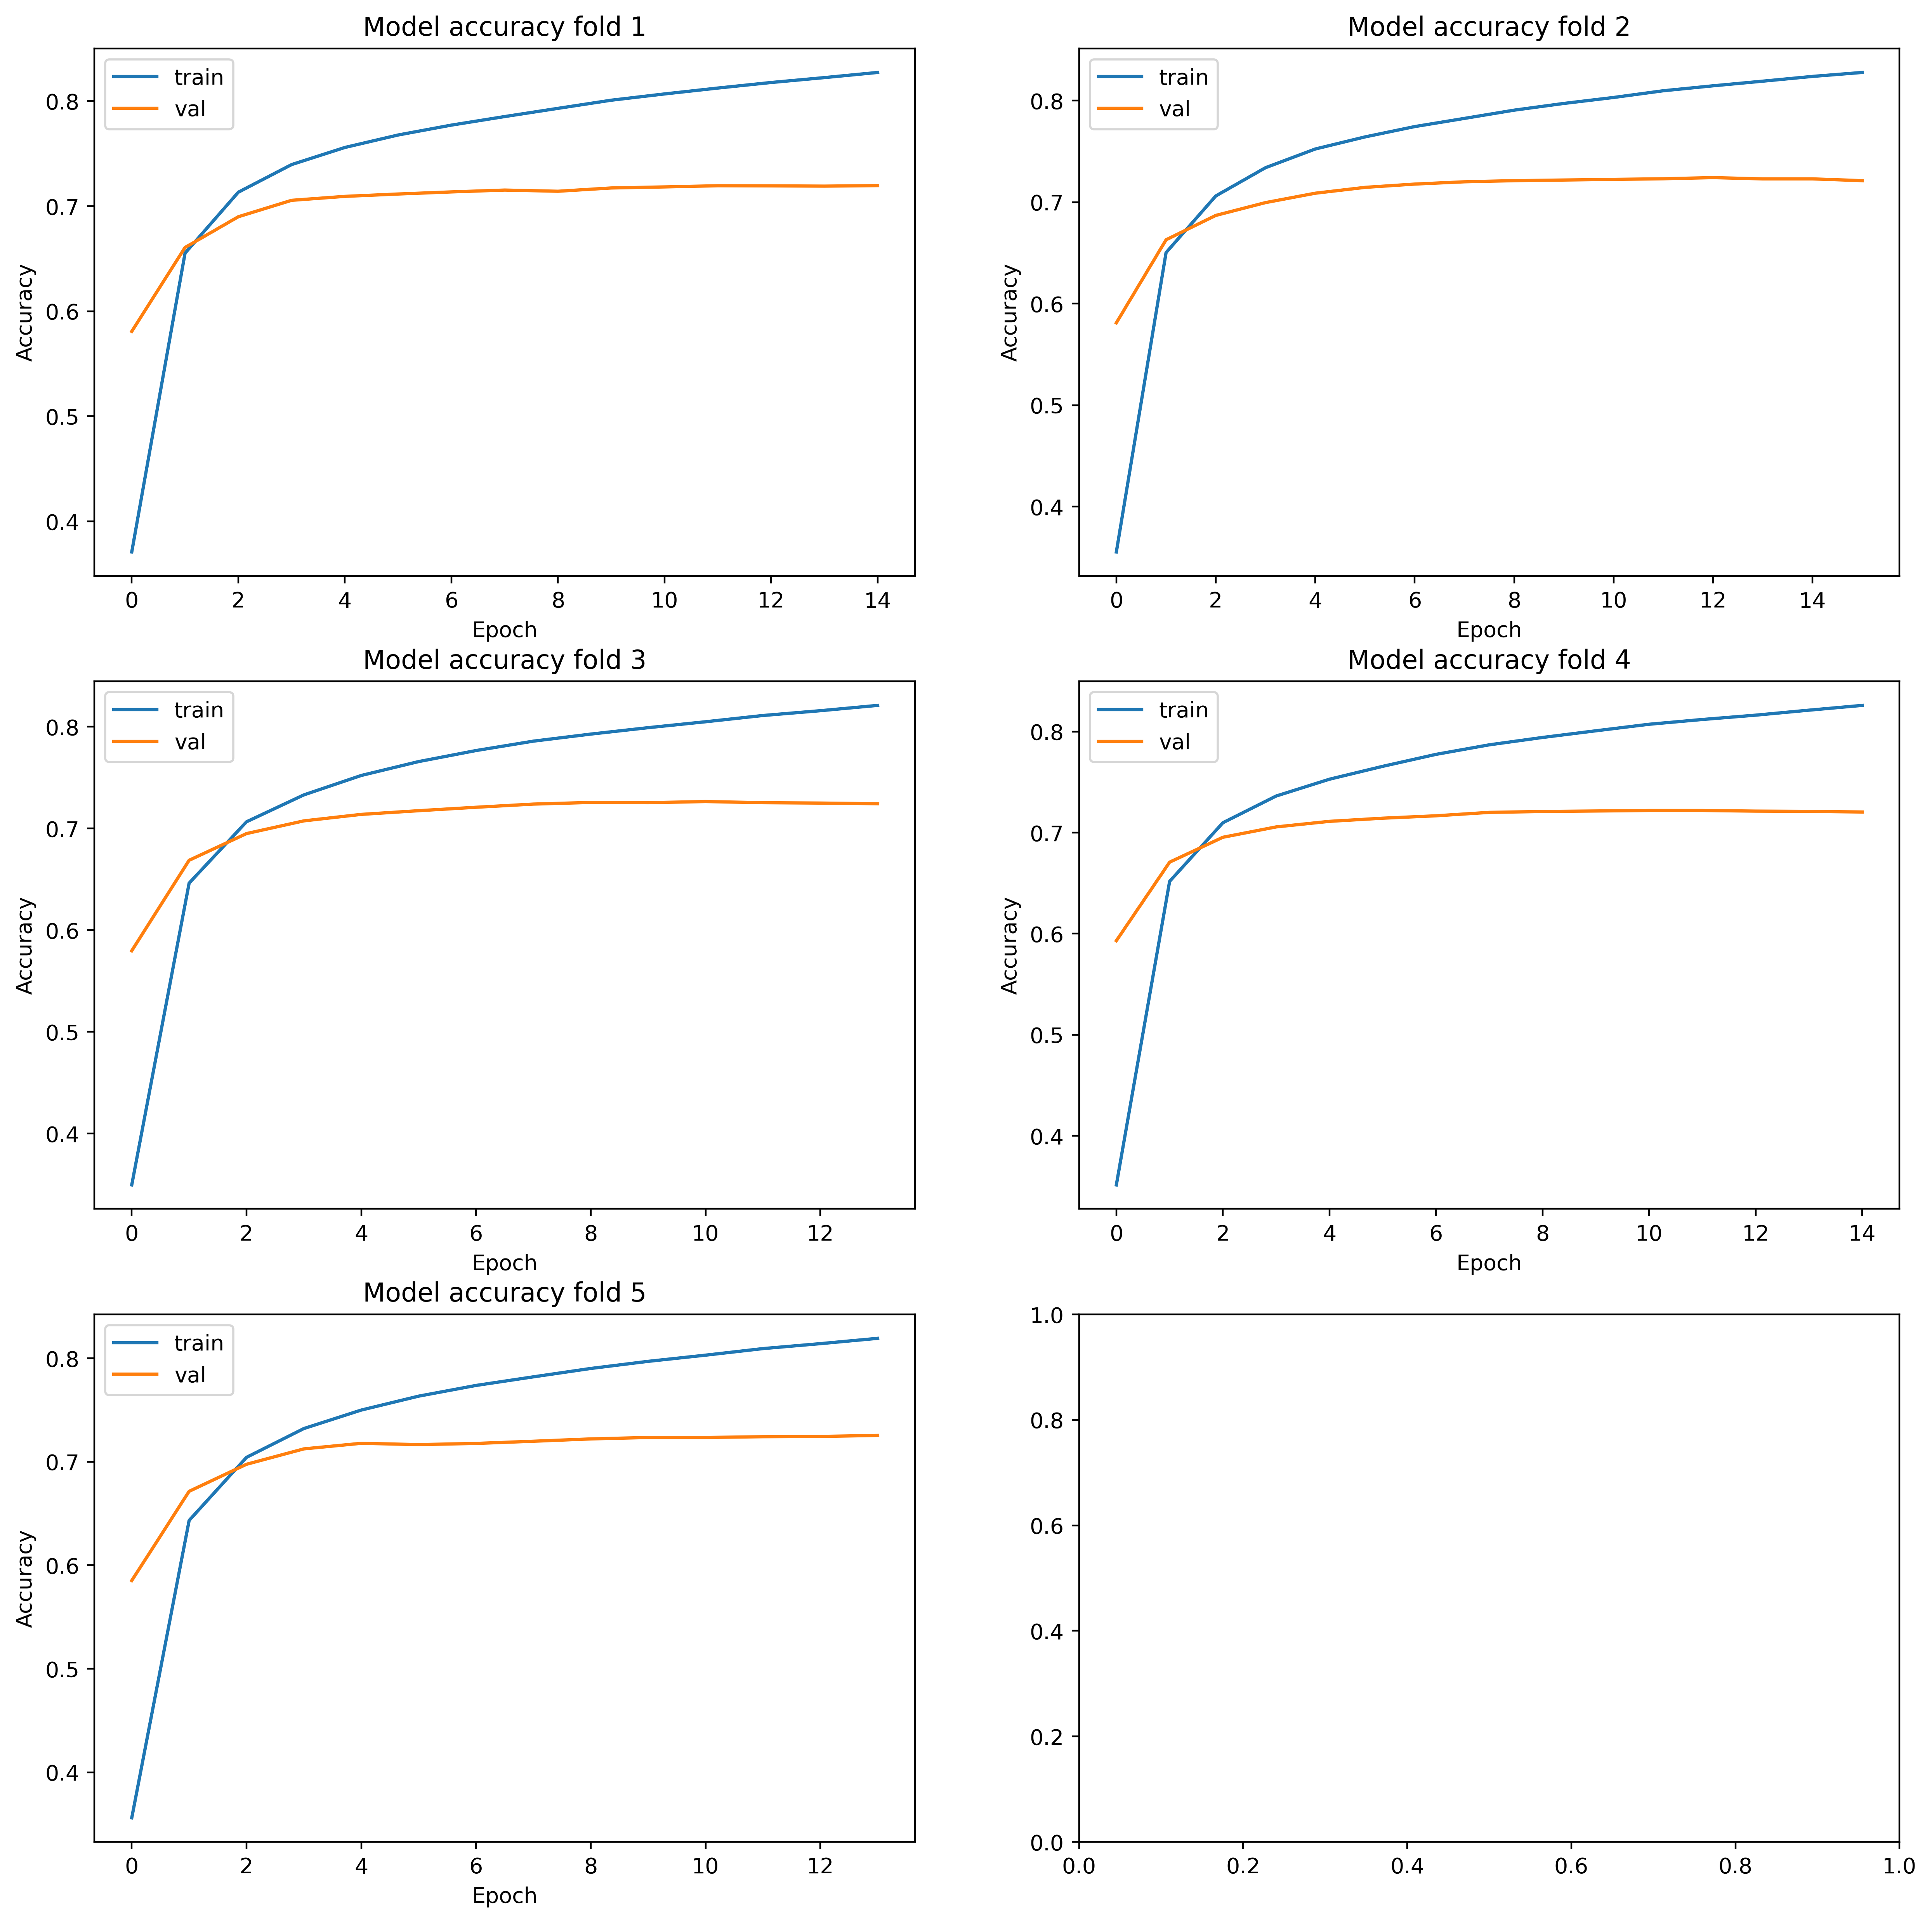
\includegraphics[width=0.5\textwidth,keepaspectratio]{figures/merged_fold_graphics_first.png}
\caption{\textit{Accuracy function} de cada \textit{fold}}
\label{diagram:accuracy_fold_first}
\centering
\end{center}
\end{figure}

\begin{figure}[t]
\begin{center}
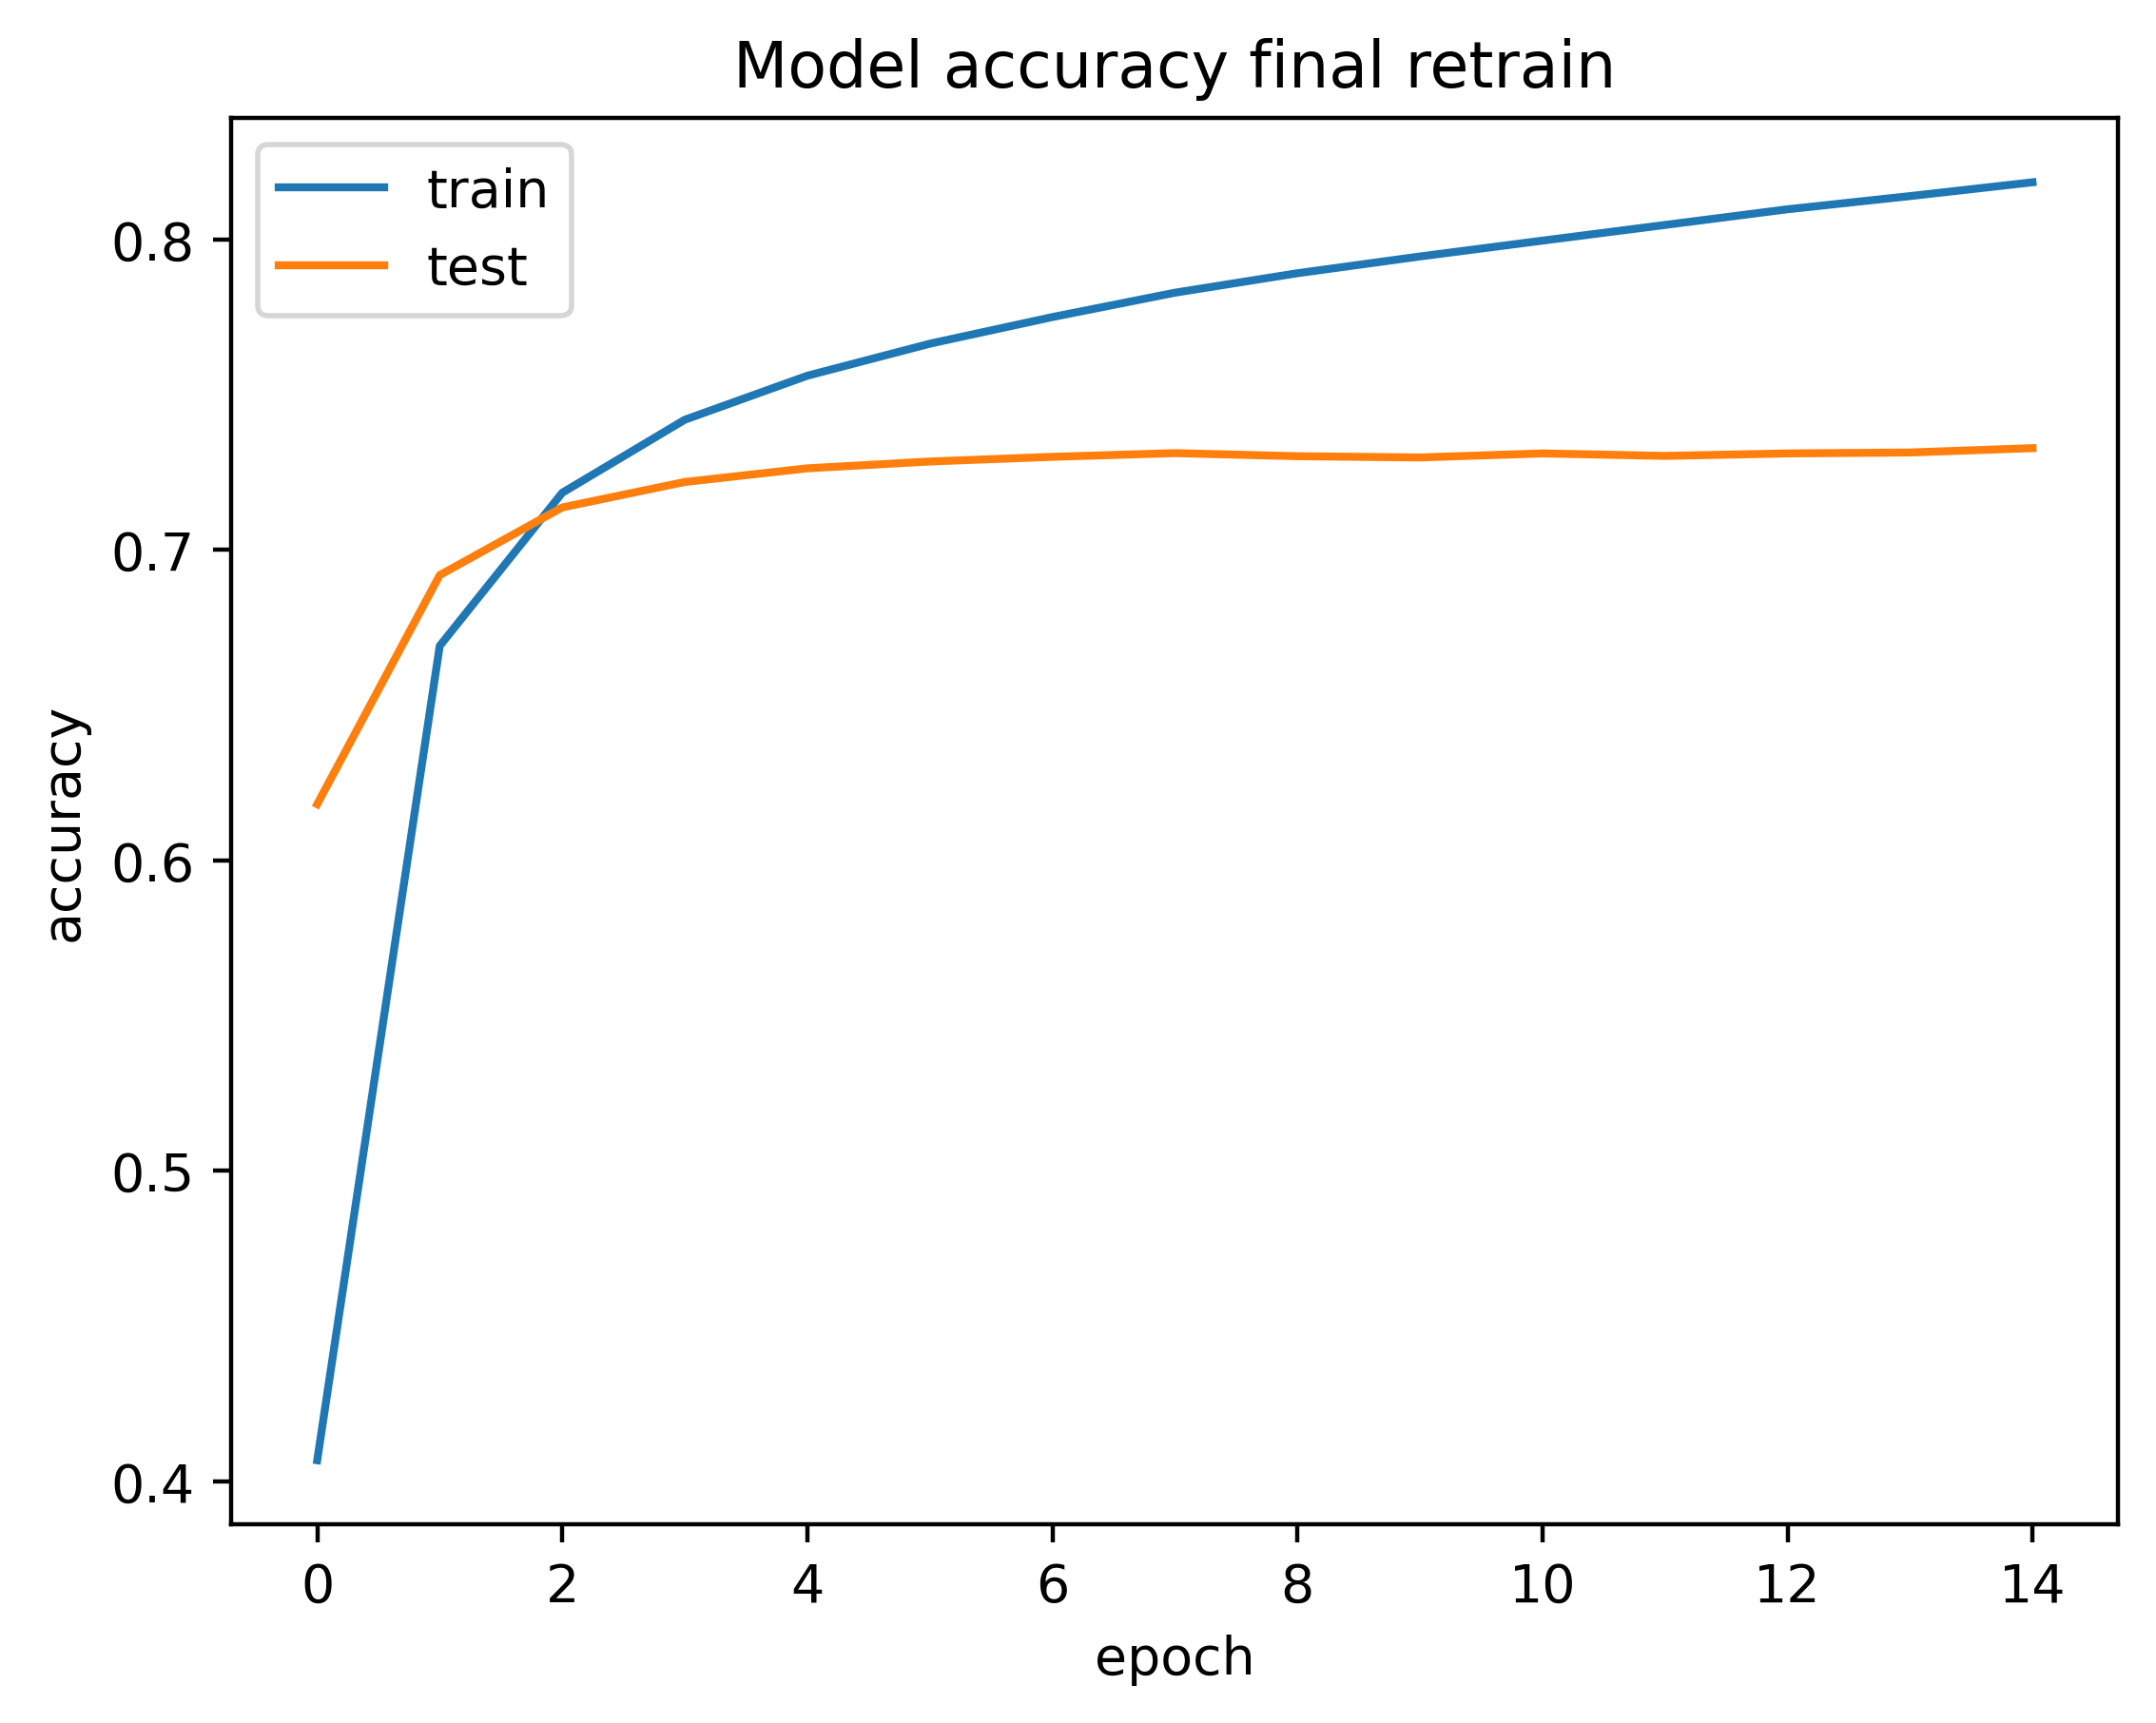
\includegraphics[width=0.5\textwidth,keepaspectratio]{figures/50_final_png_first.png}
\caption{\textit{Accuracy function} após re-treino com o conjunto de treino na totalidade}
\label{diagram:accuracy_retrain}
\centering
\end{center}
\end{figure}

\subsection{Melhoria do modelo}

Para evitar o fenómeno de \textit{overfit} decidimos acrescentar uma função de \textit{regularização} nos pesos, \textit{L2 regularization penalty} \cite{l2_regularizer}, nas \textit{hidden layers}. Basicamente a regularização evita o fenómeno de \textit{overfit}, restringindo os valores dos pesos, evitando que o modelo se adapte demasiado à forma dos dados de treino.
Para isso o algoritmo de regularização tem um parâmetro que define o impacto da regularização nos termos. Caso o valor seja muito alto, o modelo não tem flexibilidade suficiente para se formatar à forma dos dados, pelo que irá ocorrer o fenómeno de \textit{underfit}. Caso seja muito baixo, o fenómeno de \textit{overfit} pode ocorrer pois o impacto do termo regularizador é fraco.
Como se pode observar no gráfico \ref{diagram:reg_factor}, para valores muito altos do factor de regularização, o modelo não consegue generalizar os dados. O que acabou por se tornar o melhor parâmetro foi o valor de $0.001$, cuja diferença entre a \textit{accuracy} do conjunto de validação e o conjunto de treino é menor.

Os valores após retreino usando o factor de regularização óptimo definido acima são:
\begin{itemize}
        \item \textit{Train Score}: 0.82
        \item \textit{Test Score}: 0.76
\end{itemize}

Como se pode observar nos gráficos \ref{diagram:accuracy_fold_last}  e \ref{diagram:accuracy_retrain_last}, houve uma melhoria relativamente à \textit{accuracy} em dados nunca vistos pelo modelo, o que indica que o fenómeno de \textit{overfit} diminui, o que consequentemente indica que o modelo obteve uma performance melhor.



\begin{figure}[t]
\begin{center}
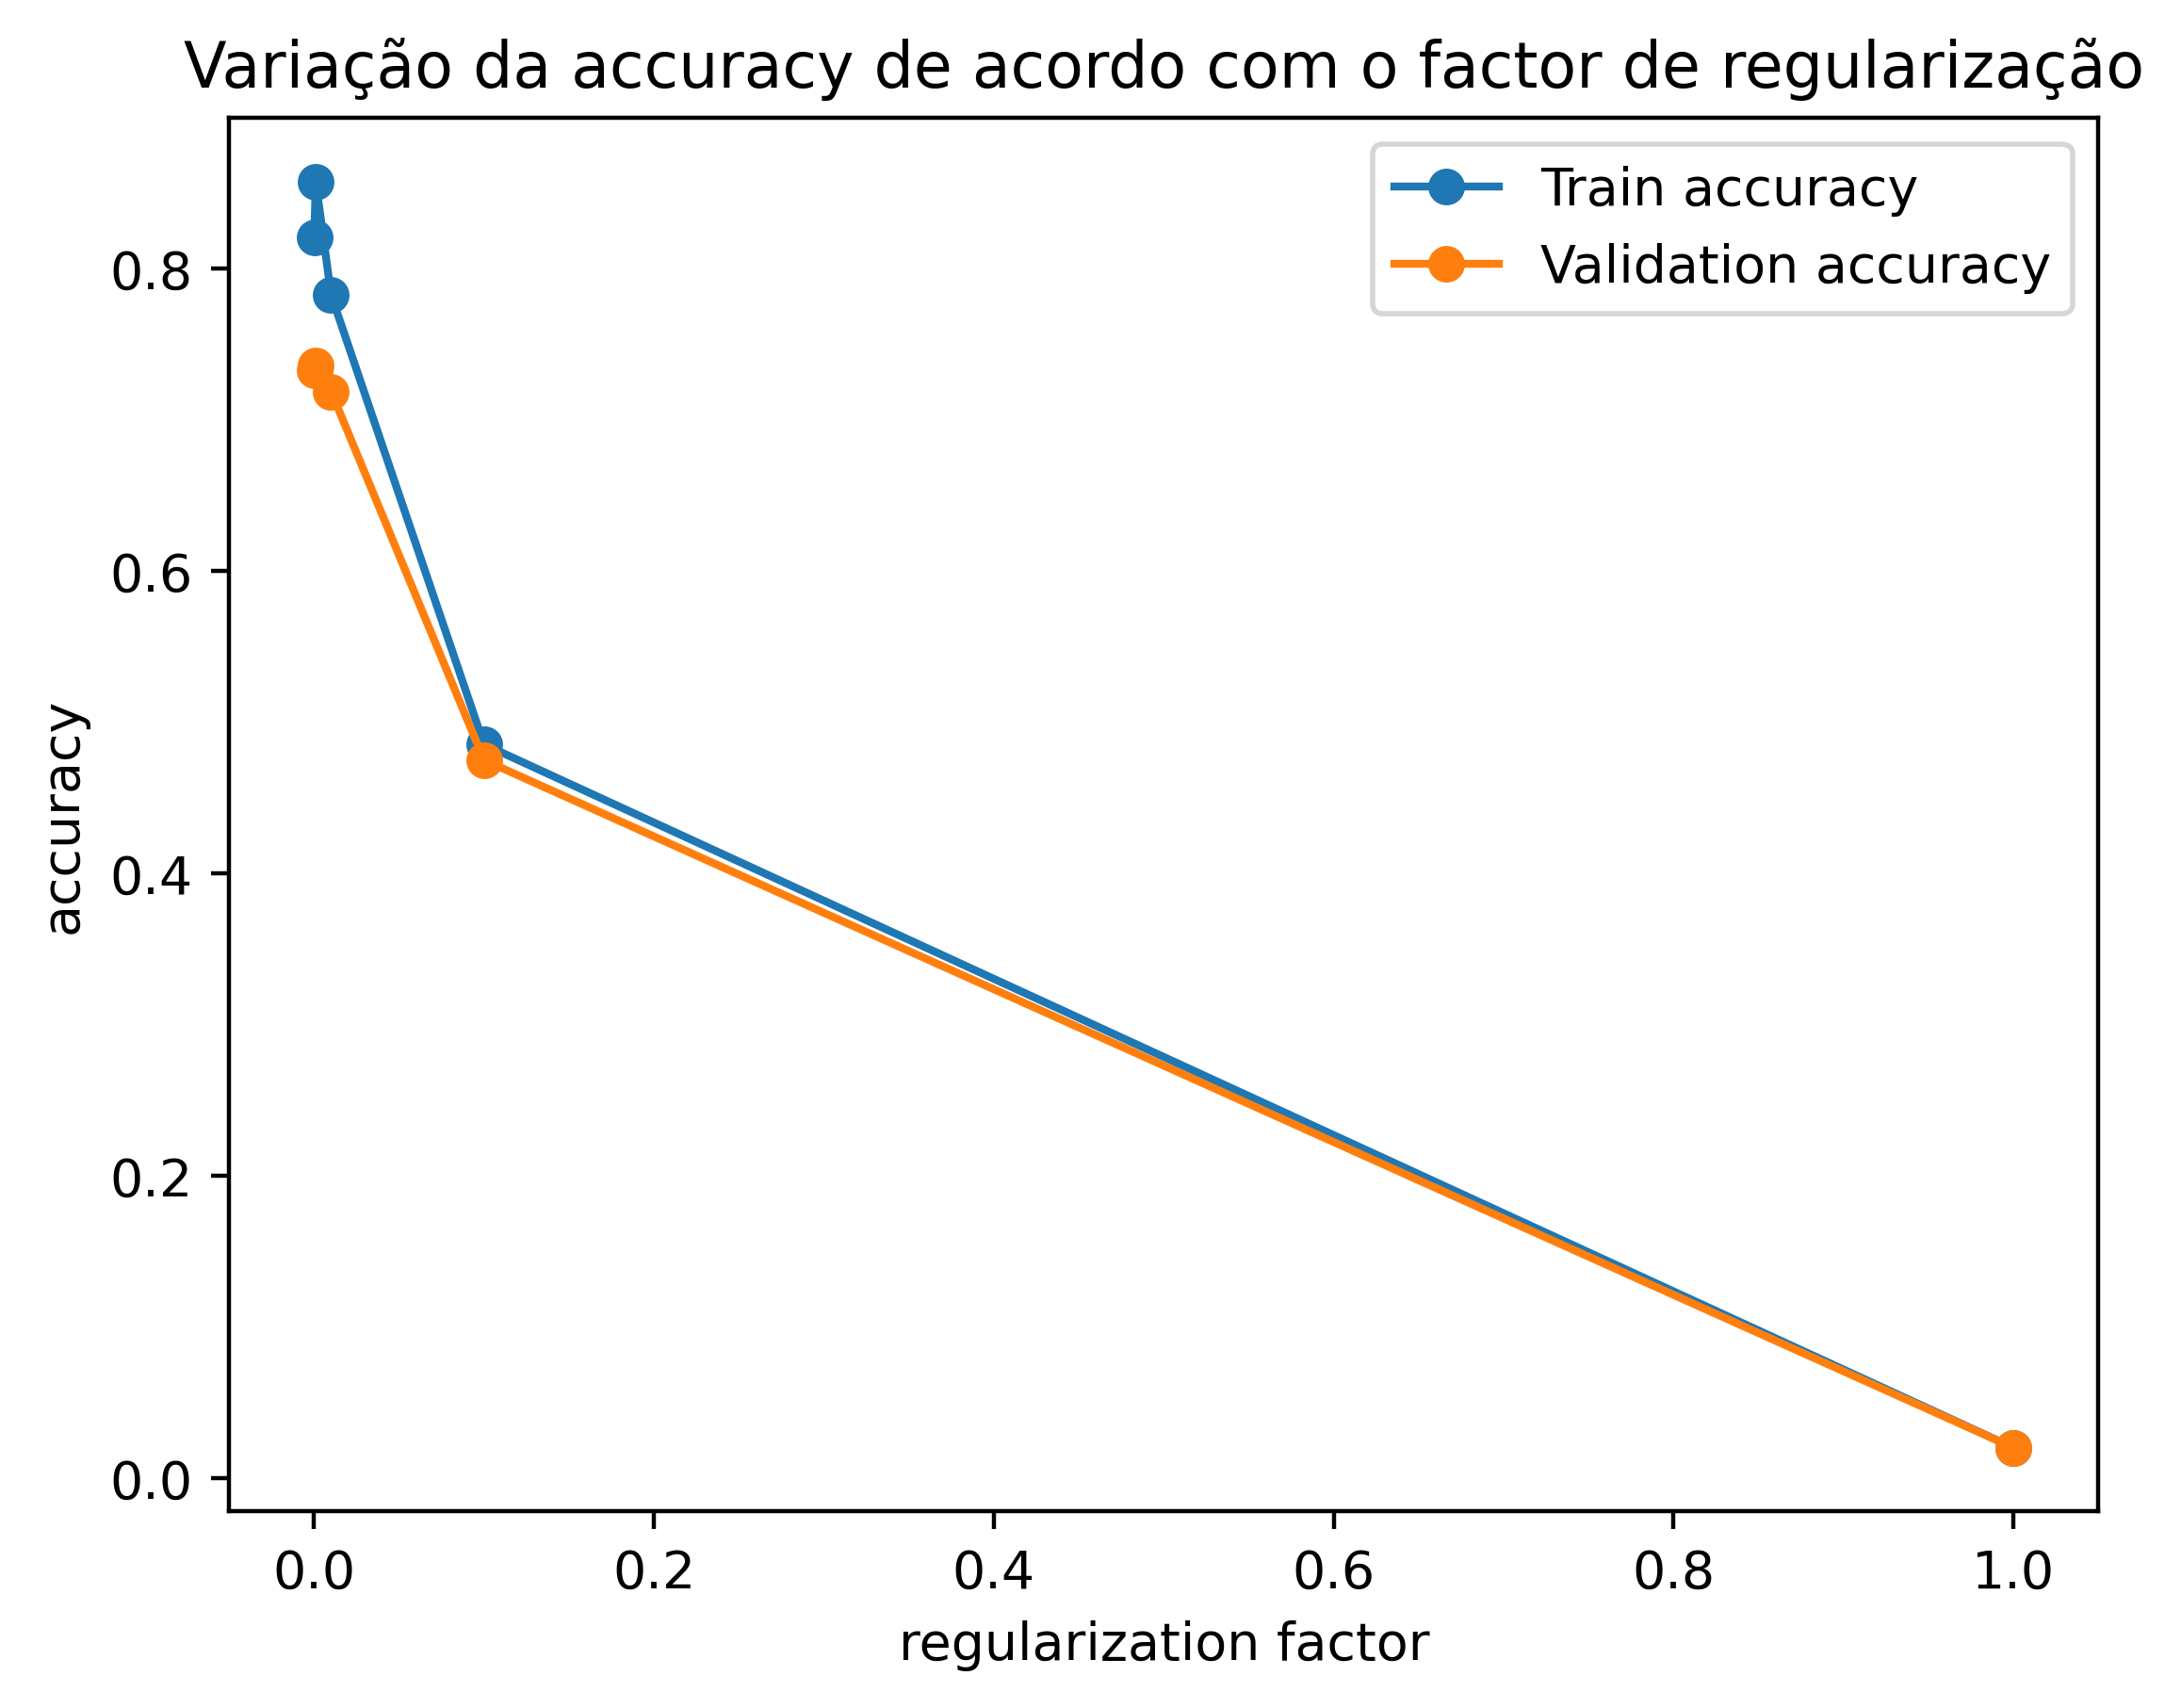
\includegraphics[width=0.5\textwidth,keepaspectratio]{figures/r_Factor.png}
\caption{Variação dos valores de \textit{accuracy} de acordo com o factor de regularização}
\label{diagram:reg_factor}
\centering
\end{center}
\end{figure}


\begin{figure}[t]
\begin{center}
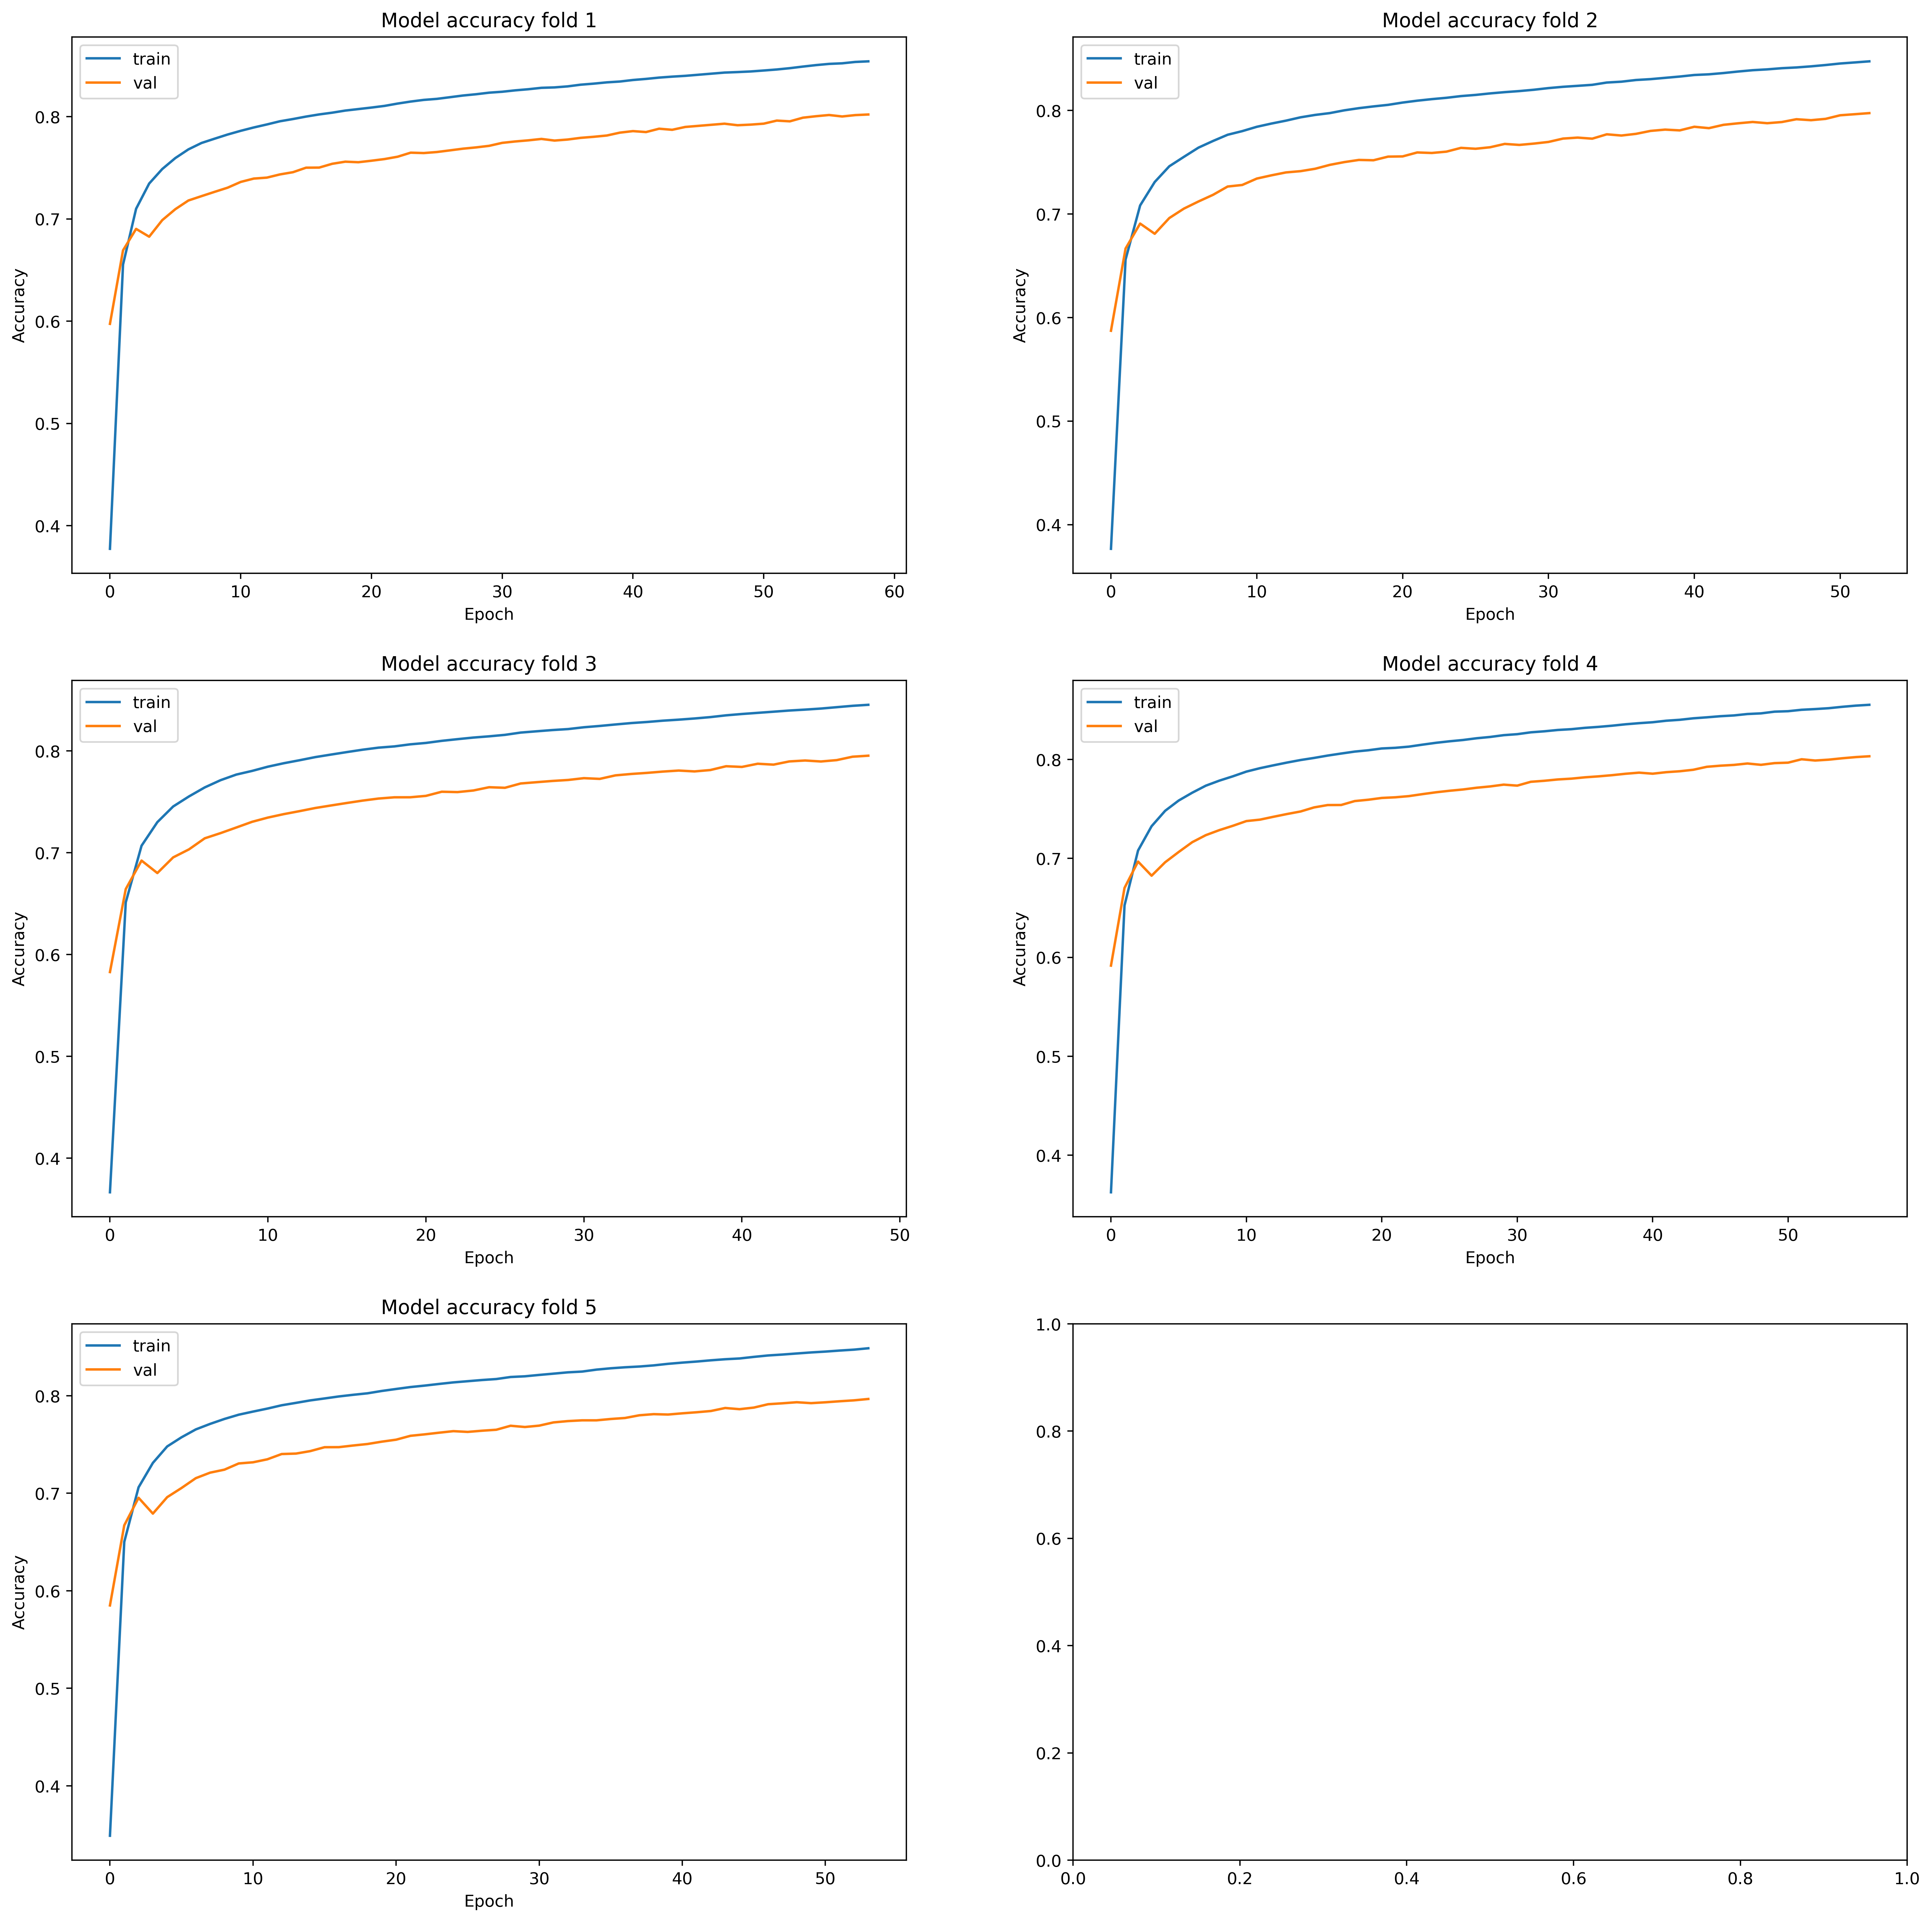
\includegraphics[width=0.5\textwidth,keepaspectratio]{figures/merged_fold_graphics_last.png}
\caption{\textit{Accuracy function} de cada \textit{fold}}
\label{diagram:accuracy_fold_last}
\centering
\end{center}
\end{figure}




\begin{figure}[t]
\begin{center}
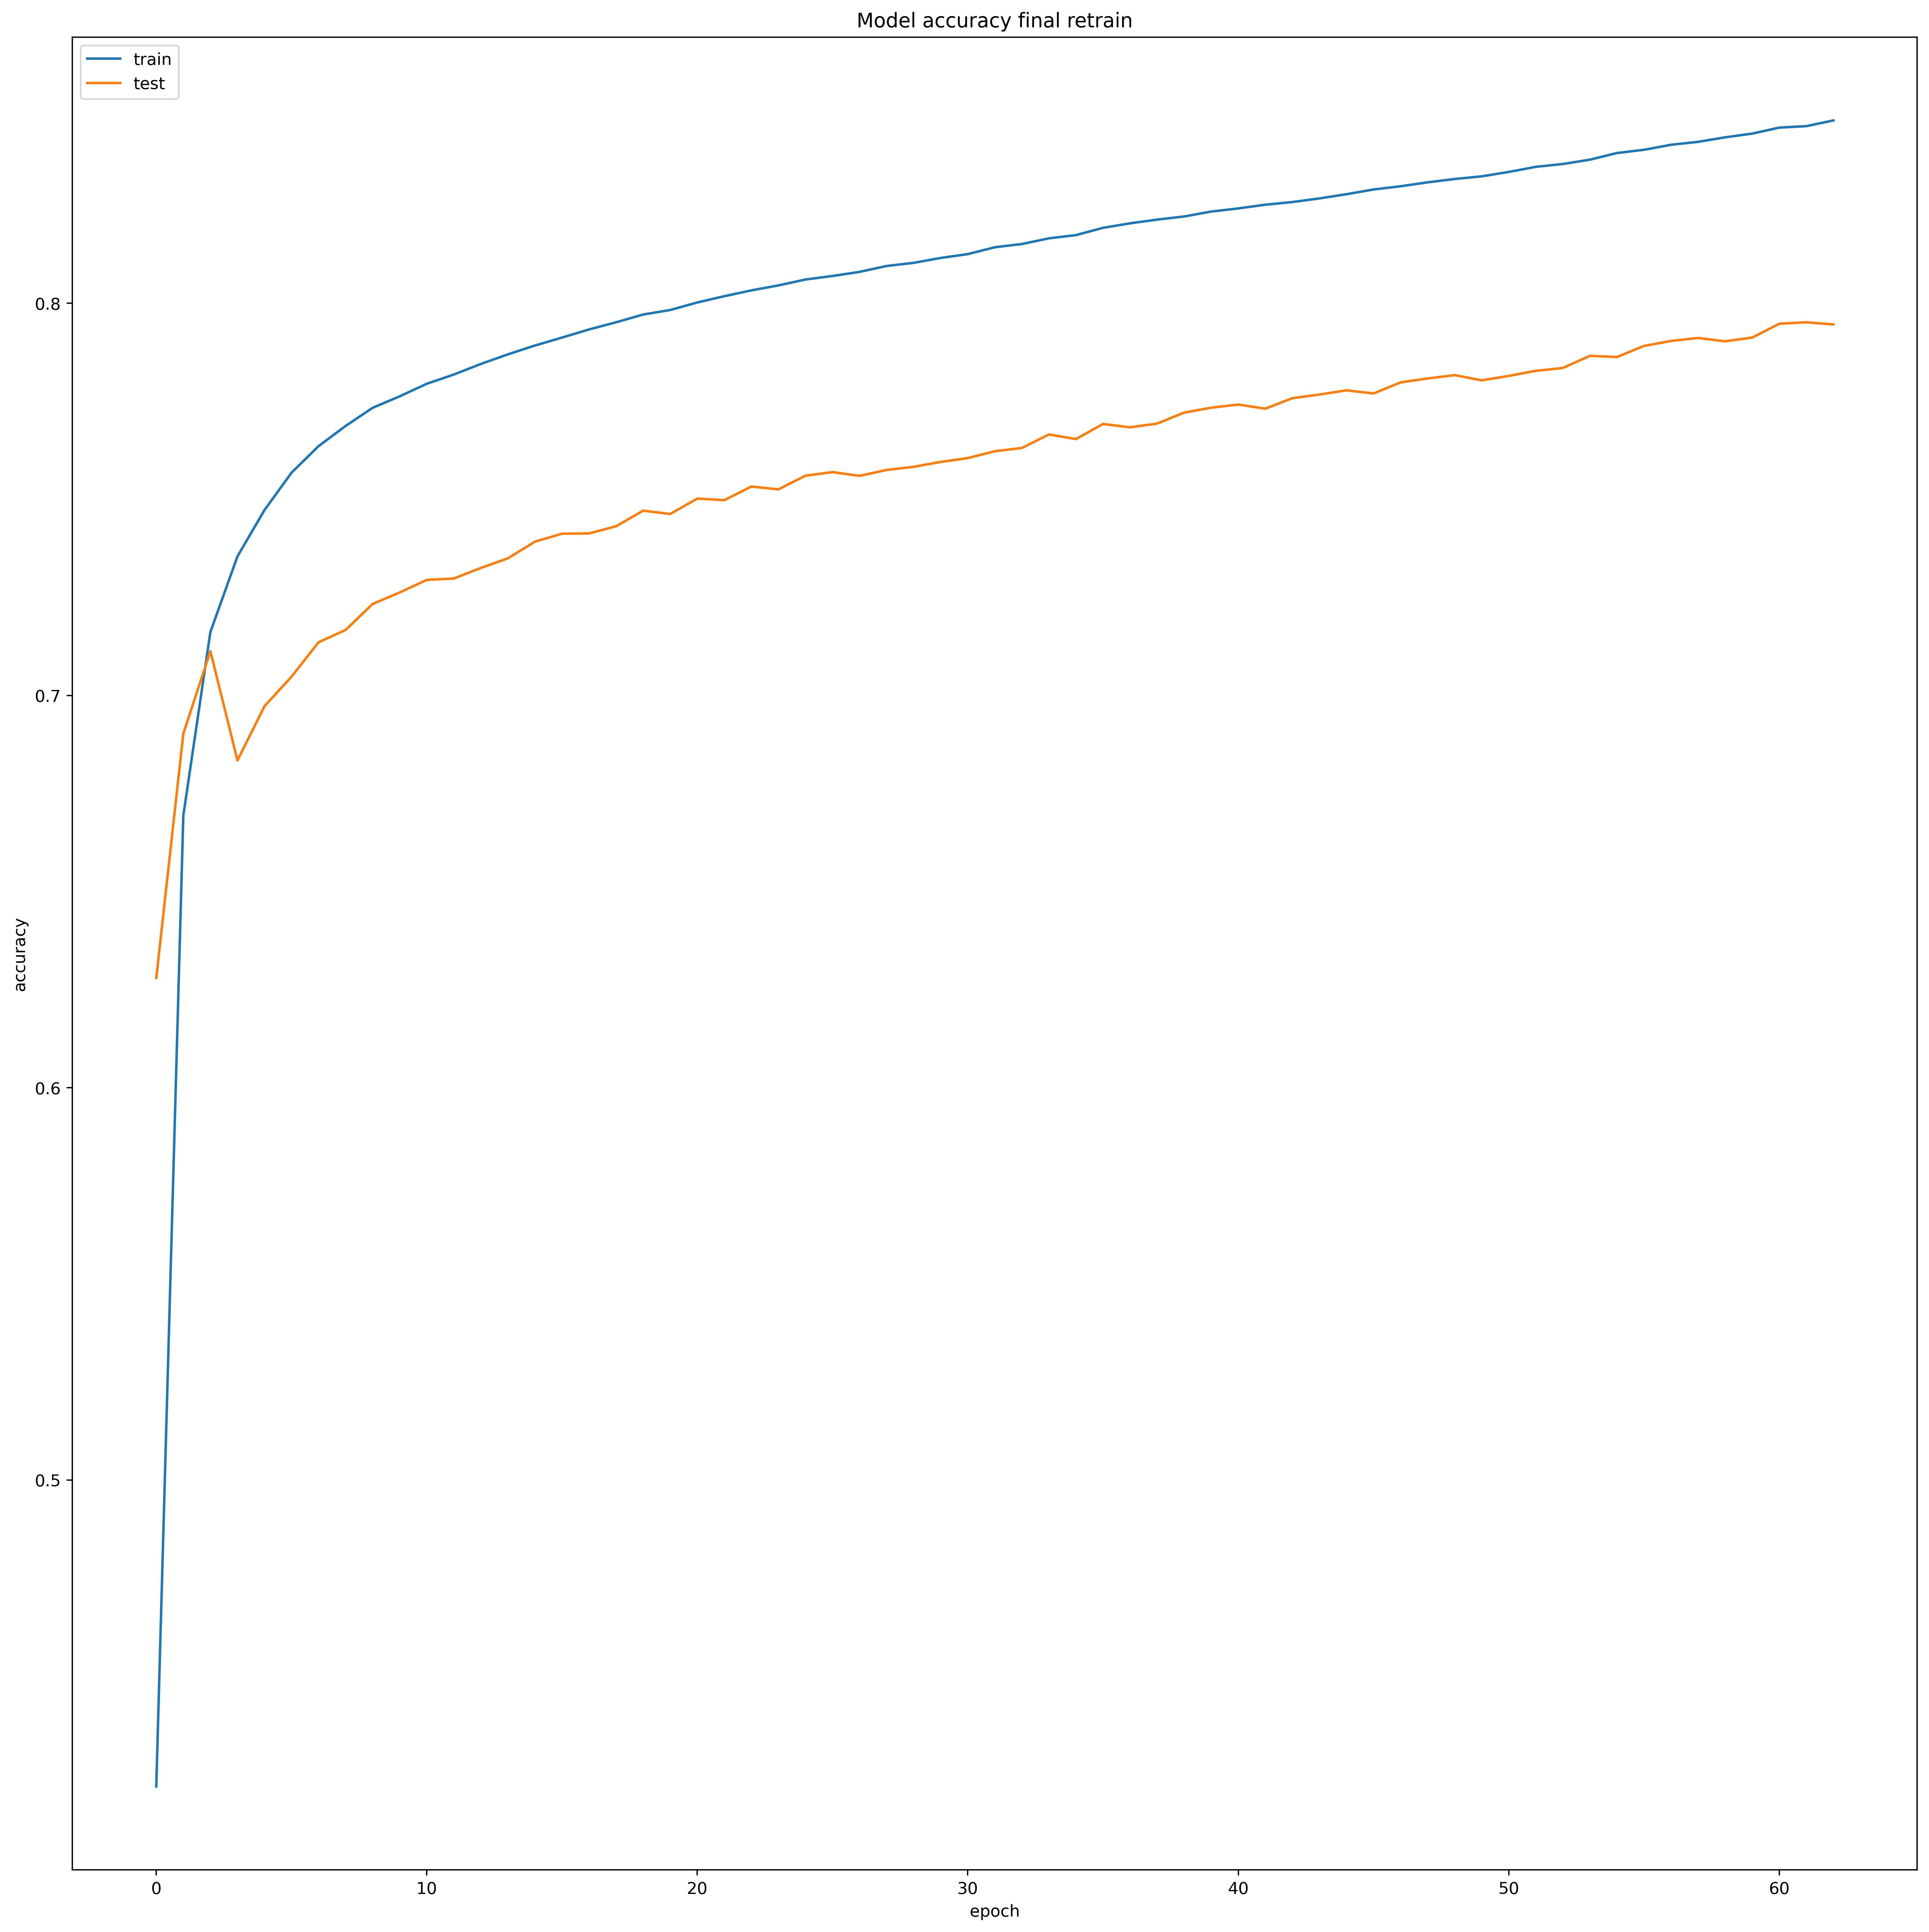
\includegraphics[width=0.5\textwidth,keepaspectratio]{figures/last_retrain.png}
\caption{\textit{Accuracy function} após re-treino com o conjunto de treino na totalidade}
\label{diagram:accuracy_retrain_last}
\centering
\end{center}
\end{figure}

\subsection{Conclusões}
Foram feitos esforços para tentar melhorar a performance deste modelo mas sem sucesso, muito devido à grande dificuldade de \textit{"fine-tune"} das redes neuronais que muito facilmente convergem para o fenómeno de \textit{overfit}.
